\documentclass[crop,tikz]{standalone}
\usetikzlibrary{backgrounds}
\colorlet{blue}{cyan}
\tikzset{
  inverted/.style = {
    color=white,
    background rectangle/.style={fill},
    show background rectangle
  }
}

\tikzset{>=latex}
\usetikzlibrary{patterns}
\colorlet{gray}{gray!60}
\colorlet{green}{green}

\begin{document}
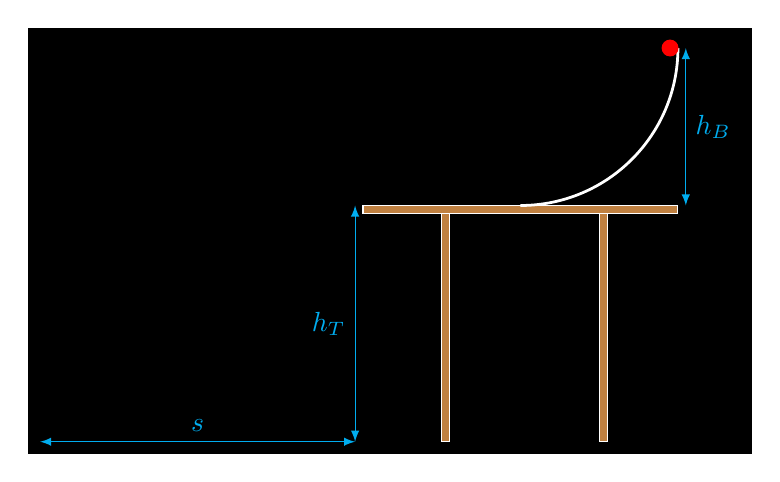
\begin{tikzpicture}[inverted,scale=2]
  \pgfmathsetmacro{\del}{0.05}
  \pgfmathsetmacro{\height}{1.5}
  % table
  \draw[fill=brown]
    (1/2,-\del) -- ++(\del,0) -- ++(0,-\height+\del) -- ++(-\del,0) -- cycle;
  \draw[fill=brown]
    (3/2,-\del) -- ++(\del,0) -- ++(0,-\height+\del) -- ++(-\del,0) -- cycle;
  \draw[fill=brown]
    (0,0) -- ++(2,0) -- ++(0,-\del) -- ++(-2,0) -- cycle;
  % track
  \draw[line width=1pt] (1,0) arc (270:360:1);
  % circle
  \coordinate (c) at (2-\del,1);
  \draw[fill,red] (c) circle (\del);
  % arrows
  \draw[blue,<->] (2.05,1) -- node[right] {$h_B$} ++(0,-1);
  \draw[blue,<->] (-\del,0) -- node[left] {$h_T$} ++(0,-\height);
  \draw[blue,<->] (-\del,-\height) -- node[above] {$s$} ++(-2,0);
\end{tikzpicture}
\end{document}
